\documentclass{sigchi-ext}
% Please be sure that you have the dependencies (i.e., additional
% LaTeX packages) to compile this example.
\usepackage[T1]{fontenc}
\usepackage{textcomp}
\usepackage[scaled=.92]{helvet} % for proper fonts
\usepackage{graphicx} % for EPS use the graphics package instead
\usepackage{balance}  % for useful for balancing the last columns
\usepackage{booktabs} % for pretty table rules
\usepackage{ccicons}  % for Creative Commons citation icons
\usepackage{ragged2e} % for tighter hyphenation

% Some optional stuff you might like/need.
% \usepackage{marginnote} 
% \usepackage[shortlabels]{enumitem}
% \usepackage{paralist}
% \usepackage[utf8]{inputenc} % for a UTF8 editor only

% Paper metadata (use plain text, for PDF inclusion and later
% re-using, if desired).  Use \emtpyauthor when submitting for review
% so you remain anonymous.
\def\plaintitle{WearLoc: A Wearable Indoor Localization Device} \def\plainauthor{Rick Gelhausen, Jennifer Nist, Lukas Gemein, David Speck
  , Andre Biedenkapp}
\def\emptyauthor{}
\def\plainkeywords{Authors' choice; of terms; separated; by
  semicolons; include commas, within terms only; required.}
\def\plaingeneralterms{Documentation, Standardization}

\title{WearLoc: A Wearable Indoor Localization Device}

\numberofauthors{5}
% Notice how author names are alternately typesetted to appear ordered
% in 2-column format; i.e., the first 4 autors on the first column and
% the other 4 auhors on the second column. Actually, it's up to you to
% strictly adhere to this author notation.
\author{%
  \alignauthor{%
    \textbf{Lukas Gemein}\\
    \email{gemeinl@cs.uni-freiburg.de} }\alignauthor{%
    \textbf{Jennifer Nist}\\
    \email{nistj@cs.uni-freiburg.de} } \vfil \alignauthor{%
    \textbf{Rick Gelhausen}\\
    \email{rick.gelhausen@gmail.com} }\alignauthor{%
    \textbf{David Speck}\\
    \email{speckd@cs.uni-freiburg.de} } \vfil \alignauthor{%
    \textbf{Andre Biedenkapp}\\   
    \email{biedenka@cs.uni-freiburg.de}}} 

% Make sure hyperref comes last of your loaded packages, to give it a
% fighting chance of not being over-written, since its job is to
% redefine many LaTeX commands.
\definecolor{linkColor}{RGB}{6,125,233}
\hypersetup{%
  pdftitle={\plaintitle},
%  pdfauthor={\plainauthor},
  pdfauthor={\emptyauthor},
  pdfkeywords={\plainkeywords},
  bookmarksnumbered,
  pdfstartview={FitH},
  colorlinks,
  citecolor=black,
  filecolor=black,
  linkcolor=black,
  urlcolor=linkColor,
  breaklinks=true,
}

% \reversemarginpar%

\begin{document}

\maketitle

% Uncomment to disable hyphenation (not recommended)
% https://twitter.com/anjirokhan/status/546046683331973120
\RaggedRight{} 

\section{Introduction}
Firefighters and other rescue teams often have to examine buildings or tunnels to find and save survivors of tragic events. Therefore they need to enter unknown environment where it can be hard to not lose the orientation. Even if the rescue team has a map of the building, it can be difficult to share the position of a located survivor with other members of the team, since ways can be blocked or impassible due destructions. It would be desirable to create maps of the surroundings that are up-to-date, which could make the work for rescue teams much easier and safer.\\
Another area of application for a wearable mapping device would be the exploration of caves, to simplify and secure the work of cave explorers.\\
In the Wearable Computing Systems lab course, we created two versions of a wearable device to create live-maps. The main difference of the versions lie in the hardware we used. Our first version is using a raspberry PI and the RPLIDAR laser scanner, which makes it a cheap and an easy to rebuild system. In the second step we tried to create a handier and even more powerful version using an Intel Edison and the Hokuyo laser scanner.\\

\newpage
\section{Hardware}
\subsection{Raspberry Pi}
The Raspberry PI 2 Model B features a 900MHz quad-core CPU and 1GB of RAM. We use the Raspberry Pi in our first setup to run the entire software for IMU and laser scanner as well as a SLAM approach. Since the Raspberry Pi lacks a display we send the results to an external device to visualize the map using a Wi-Fi network.

\subsection{Intel Edison}
The Intel Edison features a 500MHz CPU and 1GB of RAM, which we use in our second version. It also runs the software for IMU and laser scanner but sends the data to an external device which runs the SLAM approach and is also used for visualization.

\subsection{Laser-Scanner Robo Peak}
The RPLIDAR is a 360 degree 2D laser scanner. The scan range expands from 0.2 to 6m. Due to its relatively large rotating part and the associate motor, the RPLIDAR is quite big for a wearable device, having a surface of about 70x100 $mm^2$. We use it in our first setup mounted on a one-handed portable platform.

\subsection{Laser-Scanner Hokuyo}
The Hokuyo laser scanner has a 240 degree measurement radius. The scan range expands from 0.02 to 4m. With its 40x40 $mm^2$ surface it is ideal to be mounted on a GoPro holder, which allows hundreds of different possible wearable designs e.g. on the head.

\subsection{Grove-IMU}
The Grove IMU 9DOF v2.0 features a gyroscope, a magnetometer and a accelerometer. We use the Grove-IMU in both our setups to measure the bearing of the laser scanners to track user rotation. Furthermore, it helps to better predict the location.

\section{Software}
Both the Raspberry Pi and the Intel Edison run the Robot Operating System (ROS), which is an open source and free to use software. Our project is based on a ROS package which implements an approach for indoor SLAM. The package is called hector\_slam and was implemented by Team Hector of the University of Darmstadt. We also use the already existing packages i2c\_imu, rplidar\_ros and urg\_node and adapted them to our needs to conveniently use the IMU as well as the laser scanners. Additionally, we used a binary blob which is uploaded onto the IMU to directly convert the raw measurements to Quaternions which were then forwarded and used in the SLAM implementation. We used a Wi-Fi network to wirelessly transfer data between the wearable and the external device used for visualization. 

\section{Wearbale v1}
In our first version we used the Raspberry PI, the IMU and the RPLIDAR laser scanner. We chose to start with the Raspberry Pi, since it offers an easy start due to its numerous ports to connect other devices. The IMU was connected using the I2C GPIO pins of the Raspberry Pi whereas the laser scanner could be easily connected through a USB port. This fast setup allowed us to get familiar with the use of the IMU and the RPLIDAR, have a look at raw data and already start adapting the code. Finally, the Raspberry Pi runs all Software components itself, including the packages for IMU and RPLIDAR as well as the SLAM approach. The map is wirelessly transferred to a laptop which is used for visualization. All the hardware components are mounted onto a wooden plate which is screwed on a aluminium table leg which is used to hold the device. Since the Raspberry Pi and the laser scanner are relatively small this version is not quite as handy which is why we created a second version.

\section{Wearable v2}
The Intel Edison does not offer GPIO pins or USB ports to directly connect our sensors which is why we designed a circuit board that holds the Intel Edison and offers the appropriate ports. The making of the board took some time, which is why we already started developing the software using the Raspberry Pi. Since the Hokuyo laser scanner is very small, we chose it over the RPLIDAR and also hoped for an improvement in the mapping result. In contrast to the Raspberry Pi, the Intel Edison runs a lightweigth version of ROS which was built from source. Since the hector\_slam package requires for a lot of dependencies and since we ran out of memory, we only installed the packaged necessary for the sensors. The SLAM approach as well as the visualization run on a laptop that receives the sensor data wirelessly. The Hokuyo laser scanner is small enough to be mounted on a 3D printed platform that can be attached to GoPro camera holders. The IMU is attached to the bottom of the platform. As there is an enormous amout of different GoPro camera holders, this allows us to attach the laser scanner and the IMU in many different ways e.g. as a helmet lamp which leaves both hands free for other tasks. We also created a 3D printed box, s.t. the Intel Edison can safely be transported and used in the pants pockets. 
%TODO ADD PICTURES OF BOTH SETUPS
%\begin{figure}
%  \includegraphics[width=0.9\columnwidth]{}
%  \caption{Insert a caption below each figure.}~\label{fig:sample}
%\end{figure}

\section{Results}
We managed to obtain satisfying results using both of our versions. We noticed that even though the resolution of the Hokuyo laser scanner is higher than the resolution of the RPLIDAR, we obtained better results using the RPLIDAR, which could be due to the limited range of 4 meters. The RPLIDAR has a range of 5.5 meters and therefore returns more reference points to better estimate the location. We think that we can significantly improve our results if we use an even more powerful scanner.
\begin{figure*}
	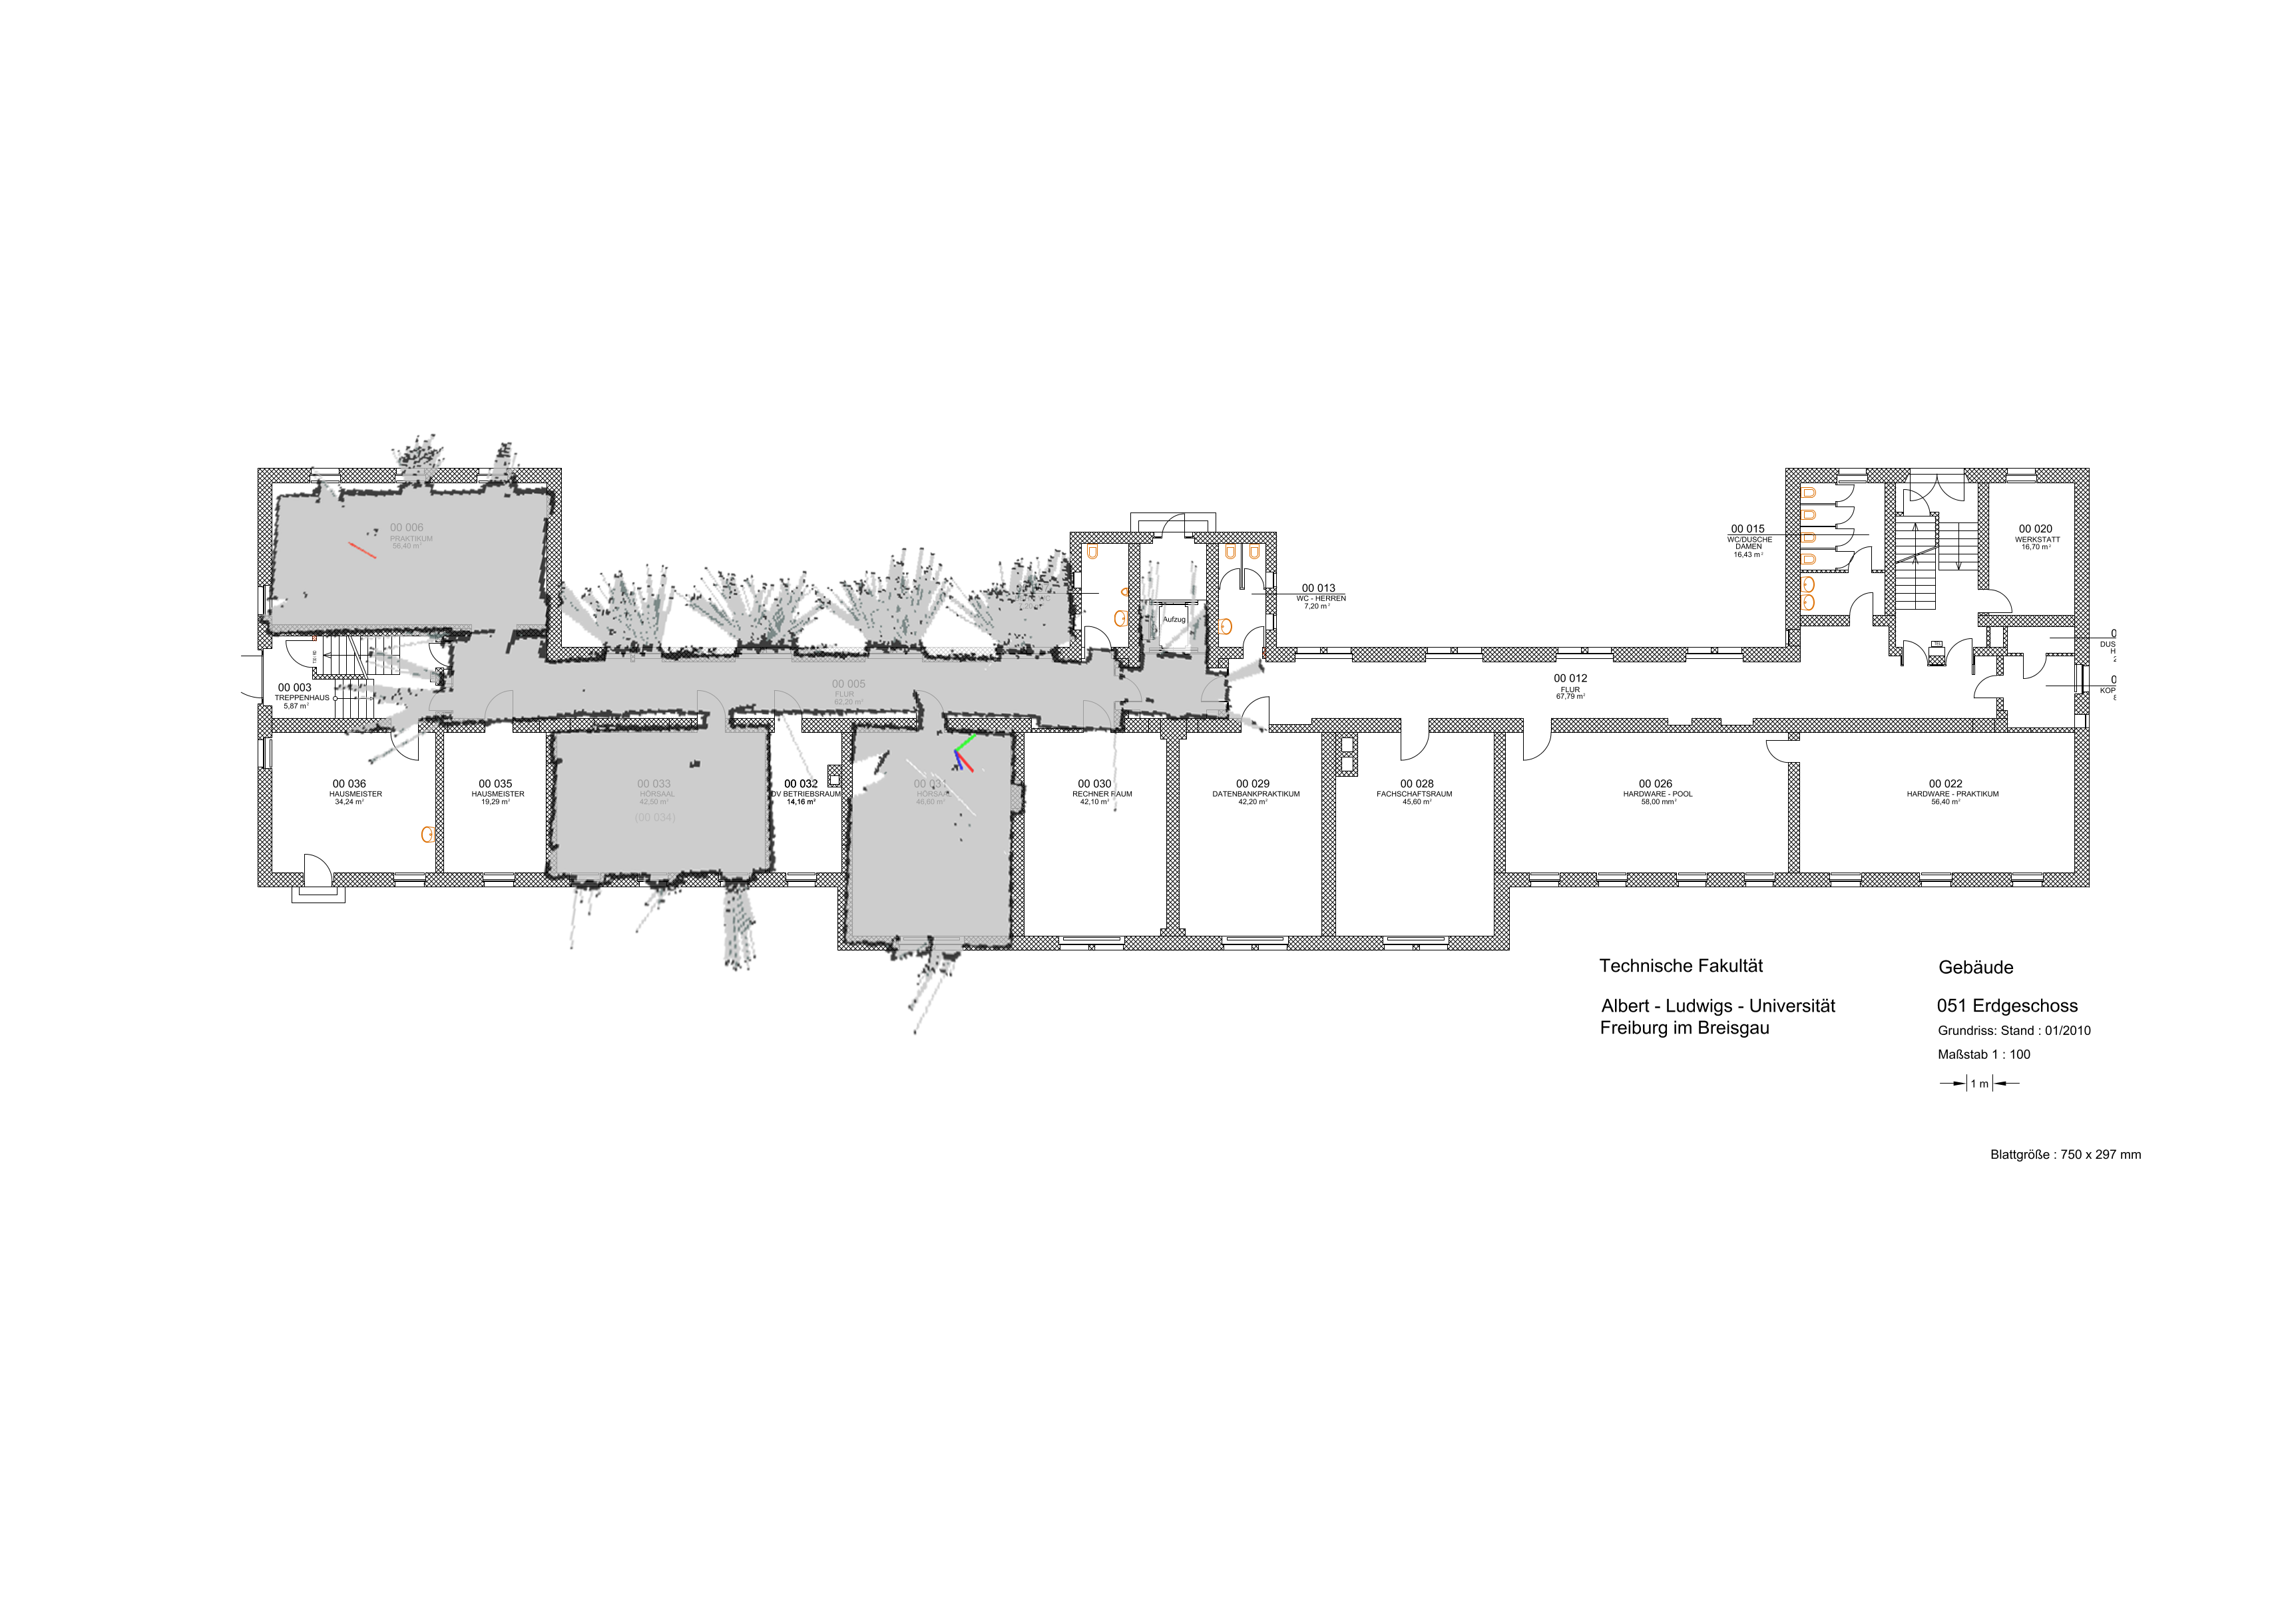
\includegraphics[width=\textwidth]{51.png}
	\caption{University of Freiburg. Mapped overlay of a part pf Building 51.}~\label{fig:b51map}
\end{figure*}
As seen in figure \ref{fig:b51map} we already get useful results using our laser-scanners. 
%\bibliographystyle{SIGCHI-Reference-Format}
%\bibliography{sample}

\balance{} 
\end{document}